\section{Results}

\subsection{Main Reasoning Results}
Table~\ref{tab:full-results} summarizes zero-shot and few-shot performance on 13 commonsense and mathematical reasoning benchmarks. Despite being 25\% smaller (1.3\,B vs.\ 1.7\,B parameters) and trained with 96 \% fewer tokens (1.4\,T vs.\ 36\,T), Xmodel-2.5 closes 71\% of the gap to Qwen3—raising the 1--2\,B average from 50.34\% (Xmodel-2) to \textbf{52.49\%}, +2.15 pp. This result is only 4.47 pp behind Qwen3 (56.96\%), confirming that the WSD schedule extracts superior reasoning efficiency per parameter and per token.

\begin{table*}[ht]
\centering
\footnotesize
\setlength{\tabcolsep}{3.5pt}
\renewcommand{\arraystretch}{1.1}
\begin{tabular}{lccccccccc}
\toprule
\textbf{Dataset (shots)} & \textbf{Qwen3} & \textbf{MiniCPM} & \textbf{InternLM2.5} & \textbf{Llama-3.2} & \textbf{Gemma-3} & \textbf{SmolLM2} & \textbf{Xmodel-2} & \textbf{\llm} \\
\midrule
ARC-Challenge (25)  & 53.07 & 45.31 & 40.96 & 41.47 & 40.36 & 53.50 & 46.16 &  48.89 \\
ARC-Easy (25)       & 79.67 & 75.21 & 71.68 & 71.80 & 69.65 & 80.81 &  76.22 &  76.94 \\
PIQA (0)            & 72.58 & 75.19 & 73.39 & 74.16 & 72.42 & 77.58 &  75.14 &  75.95 \\
HellaSwag (10)      & 60.16 & 67.90 & 59.14 & 59.76 & 55.96 & 73.16 &  64.05 &  67.24 \\
WinoGrande (5)      & 60.54 & 64.48 & 61.88 & 61.25 & 58.48 & 67.88 &  64.25 &  64.64 \\
BBH (3)             & 45.23 & 35.45 & 41.12 & 38.10 & 38.34 & 35.05 &  48.90 &  54.58 \\
MMLU (5)            & 60.24 & 48.75 & 48.87 & 45.44 & 39.87 & 49.99 &  49.98 &  51.81 \\
GSM8k (5)           & 69.29 & 42.00 & 41.77 & 34.80 & 25.70 & 32.37 &  56.56 &  58.98 \\
MATH (4)            & 35.50 & 12.06 & 21.20 & 16.84 & 24.06 & 10.96 &  25.64 &  28.94 \\
HumanEval (0)       & 42.68 & 43.90 & 35.98 & 31.10 & 32.93 & 25.61 &  29.27 &  28.66 \\
MBPP (3)            & 42.60 & 33.40 & 32.80 & 32.60 & 25.00 & 34.40 &  30.80 &  33.00 \\
CMMLU (5)           & 60.47 & 46.52 & 62.03 & 36.99 & 34.11 & 33.60 &  44.29 &  47.16 \\
C-Eval (5)          & 60.40 & 46.21 & 61.59 & 37.00 & 33.51 & 34.55 &  43.16 &  45.54 \\
\midrule
\textbf{Average}    & 56.96 & 48.95 & 50.19 & 44.72 & 42.34 & 46.88 &  50.34 &  \textbf{52.49} \\
\bottomrule
\end{tabular}
\caption{Comprehensive results (\%) on 13 benchmarks. \textbf{Bold} marks best in 1--2\,B range. \llm 1.3B uses flexible-extract for GSM8k and math\_verify for MATH.}
\label{tab:full-results}
\end{table*}

\subsection{Training Loss}
Figure~\ref{fig:loss} presents the training loss curve on the WikiText-2 dataset \citep{merity2016pointer}. The initial drop corresponds to increasing the batch size from 2M to 4M tokens, which likely replicates the stabilizing effect of a reduced learning rate \citep{smith2018batchsize}. The second drop reflects the impact of the learning rate decay phase. Immediately after decay, we conduct a lightweight long-context adaptation (shaded region in Figure~\ref{fig:loss}): starting from 550k steps, we first expand the context length from 3,712 to 8,192 within 3k steps, and then further to 16,384 within the next 7k steps. As expected, the longer-context exposure produces a small bump on WikiText-2 perplexity; nevertheless, the 13-task average in Table~\ref{tab:full-results} rises from 52.36 to 52.49, confirming that the long-context phase converts the modest perplexity increase into tangible downstream reasoning gains.

\begin{figure*}[ht]
\centering
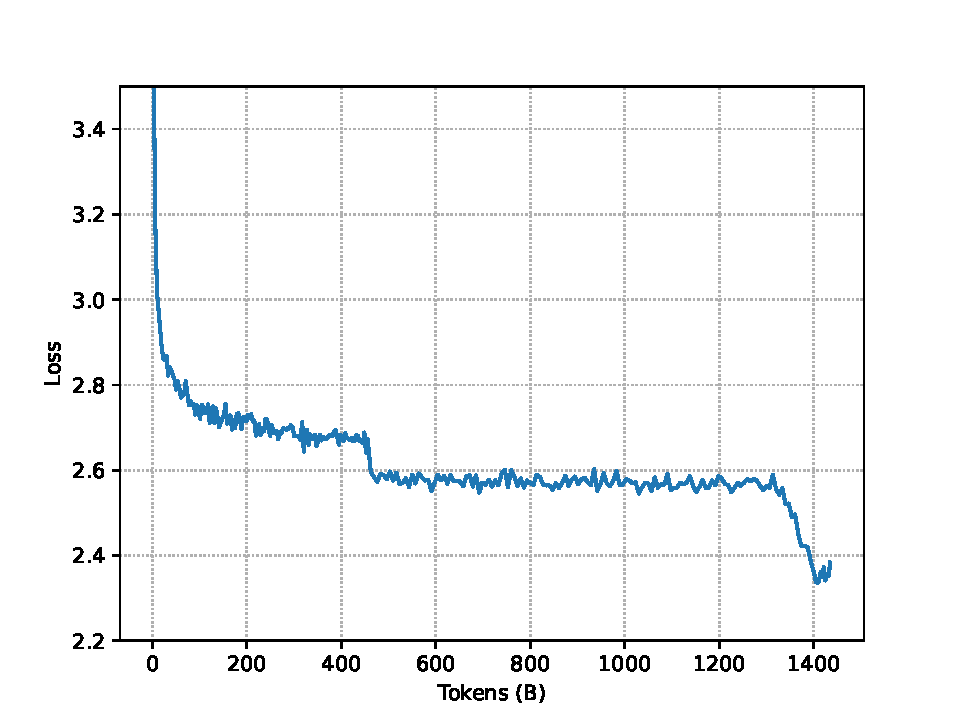
\includegraphics[width=0.8\linewidth]{figures/val_loss.pdf}
\caption{Loss curve for \llm 1.3B.}
\label{fig:loss}
\end{figure*}